\chapter{Pruning}\label{ch:pruning}
In \autoref{ch:introduction} I gave a brief explanation of few techniques for
doing model optimisation on a neural network. Pruning is one of these and in
the first part of this chapter I give a more detailed explanation.
The second part instead focuses on the pruning API in TensorFlow Model
Optimization.
This section gives the basis to fully understand the next chapter
(\autoref{ch:objective}) where I will explain the architecture of the
implementation of this technique in TensorFlow Model Optimization.

\section{What's pruning?}
Neural network pruning is the task of reducing the size of a network by
removing parameters. This compression affects the size of the model, the
latency, the amount of memory and the computational power needed to run the
inference. These metrics need to be balanced with the accuracy of the model
itself. I give a more detailed analysis about this trade-off in
\autoref{subsec:tradeoff}

Pruning has been used since the late 1980s but has seen an explosion of
interest in the past decade thanks to the rise of deep neural networks.
It sets its roots with a couple of classic papers:\textit{Optimal Brain
Damage}~\cite{lecun-90b} and \textit{Optimal Brain Surgeon}\cite{hassibi-93}

In the last decade (2010--2020) a few dozens papers have been published in
literature about pruning\cite{blalock2020state} and all of them have been
showing that pruning is an effective technique that can be applied to a variety
of neural network on different fields (image and speech recognition, text
processing, etc\ldots).
Moreover they highlights that pruning is a versatile technique as, I said
earlier, it has a positive impact on multiple metrics, all important for a
better edge deployment of the model.

How does pruning reduce the size of a model? The basic principle is to prune
(remove) unnecessary neurones or weights (see \autoref{fig:pruning_weights_neurons}):

\begin{figure}[ht]
    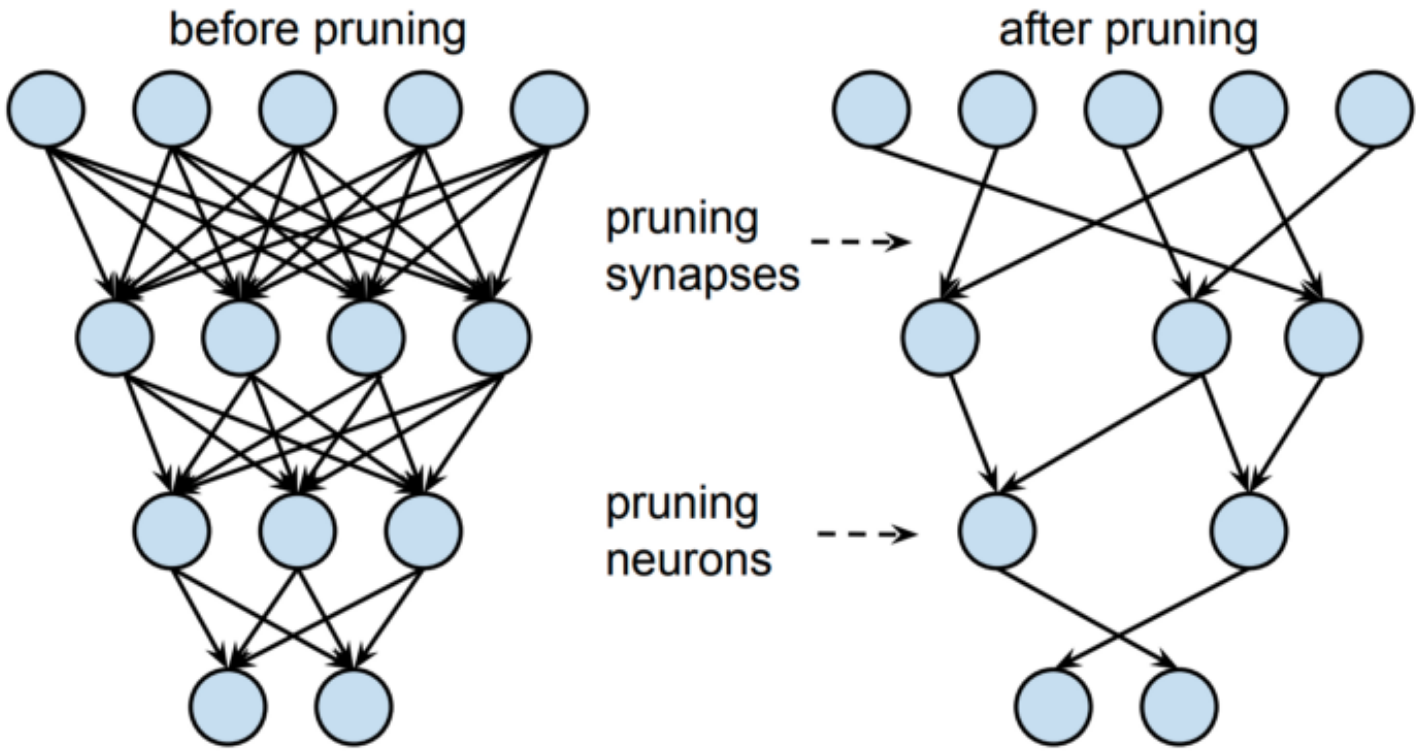
\includegraphics[width=8cm]{images/pruning/pruning_weights_neurons.png}
    \centering
    \caption{Pruning weights and neurons}\label{fig:pruning_weights_neurons}
\end{figure}

\begin{itemize}
    \item \textbf{weights}: this is done by setting individual parameters to
        zero and making the network sparse. The effect will be to maintain the
        same architecture of the network but lowering down the number of
        parameters.
    \item \textbf{neurons}: this is done by removing the entire node from the
        network with all its connections. This would make the network
        architecture smaller but with the target to keep the accuracy of the
        starting network.
\end{itemize}

\subsection{Pruning techniques}
The main problem in pruning is to understand what to prune. Of course the goal
is to remove nodes and/or weights that are less useful, i.e.\ whose removal
does not greatly affect the model performance. There are different methods to
understand what to prune with very little or no effect on accuracy.
Below a brief description of different pruning techniques is given.

\subsubsection{Magnitude Pruning}
A neural network can be expressed in many ways and functions can be a very
simple case of a neural network. Its coefficients can be changed in order to
learn the input data points.
There are coefficients that, despite changing their values, they won't change
the behaviour of the function and these are referred as
\textbf{non-significant}.
In neural networks these coefficients are weights and biases: they are
\textbf{trainable parameters} and the same non-significant concept can be
applied to them with a bit more complexity.

During the back-propagation (gradient descent) some weights are updated with
larger gradient magnitudes (both positive and negative) than the others.
These weights are the \textbf{significant} ones and the weights receiving very
small gradients can be considered as \textbf{non-significant} as their impact
is minimal to the optimization of the loss function.
After the training, the weight magnitude of every layer can be explored in
order to check which weights are significant.

The weight magnitude can then be used as a criteria for pruning the neural
network.
In this technique a \textbf{threshold} is specified and all the weights below
this threshold are considered non-significant. This is usually combined with a
\textbf{sparsity target} the network should achieve.
The \textbf{non-significant weights will be zeroed}, cancelling effectively
their impact in the neural network.
This can be applied to biases as well and, in general, to any trainable
parameter, to be precise.

Once the pruning is done it's always advisable to retrain the network in order
to compensate for any drop in performance. It's worth noticing that during the
retraining the pruned weights won't be updated.~\cite{magnitude_pruning}

Magnitude pruning is the technique I will be using in
\autoref{ch:objective}.

\subsubsection{Channel Pruning}
Channel pruning is a technique specifically for CNN (Convolutional Neural
Network) as it relies on the architecture of this type of networks.
The building blocks of a classical CNN are (see \autoref{fig:cnn}):

\begin{figure}[ht]
    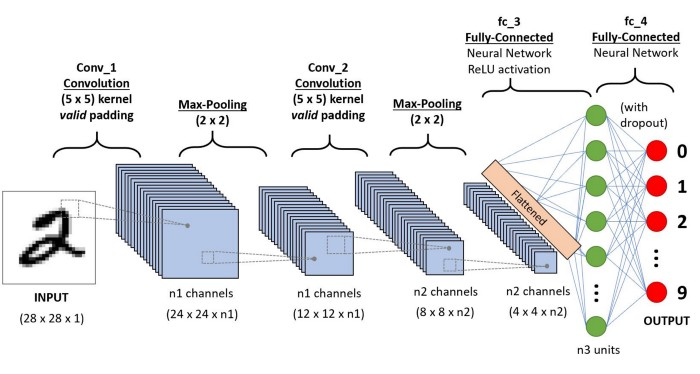
\includegraphics[width=\textwidth]{images/pruning/cnn.jpeg}
    \centering
    \caption{Convolutional neural network architecture}\label{fig:cnn}
\end{figure}

\begin{itemize}
    \item \textbf{Convolutional layer}: it is the core building block of a CNN\@.
        A convolution is the simple application of a filter to an input that
        results in an activation. Repeated application of the same filter to an
        input results in a map of activations called a feature map, indicating
        the locations and strength of a detected feature in an input, such as
        an image.
    \item \textbf{Pooling layer}: it provide an approach to down sampling
        feature maps by summarizing the presence of features in patches of the
        feature map. Two common pooling methods are average pooling and max
        pooling that summarize the average presence of a feature and the most
        activated presence of a feature respectively.
    \item \textbf{ReLU layer}: ReLU stands for \textbf{Rectified Linear Unit}
        and it is a piecewise linear function that will output the input
        directly if it is positive, otherwise, it will output zero. It has
        become the default activation function for many types of neural
        networks because a model that uses it is easier to train and often
        achieves better performance (see \autoref{fig:relu})
\begin{figure}[ht]
    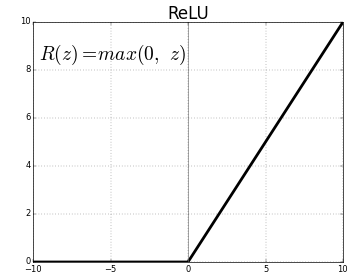
\includegraphics[width=8cm]{images/pruning/relu.png}
    \centering
    \caption{Rectified linear unit activation function}\label{fig:relu}
\end{figure}
    \item \textbf{Fully connected layer}: after several convolutional and max
        pooling layers, the high-level reasoning in the neural network is done
        via fully connected layers. Neurons in a fully connected layer have
        connections to all activations in the previous layer, as seen in
        non-convolutional artificial neural networks.
    \item \textbf{Loss layer}: it specifies how training penalizes the
        deviation between the predicted (output) and true labels and is
        normally the final layer of a neural network. Various loss functions
        appropriate for different tasks may be used. Softmax loss is used for
        predicting a single class of K mutually exclusive classes.
        Sigmoid cross-entropy loss is used for predicting K independent
        probability values in [0, 1]. Euclidean loss is used for regressing to
        real-valued labels.\cite{cnn}
\end{itemize}

\autoref{fig:channel_pruning} shows the channel pruning algorithm for a
single convolutional layer.
The aim is to reduce the number of channels of feature map B, while maintaining
outputs in feature map C.
Once the channels are pruned, corresponding channels of the filters that take
these channels as input can be removed. Moreover, filters that produce these
channels can be removed as well. It is clear that channel pruning involves
two key steps.

\begin{figure}[ht]
    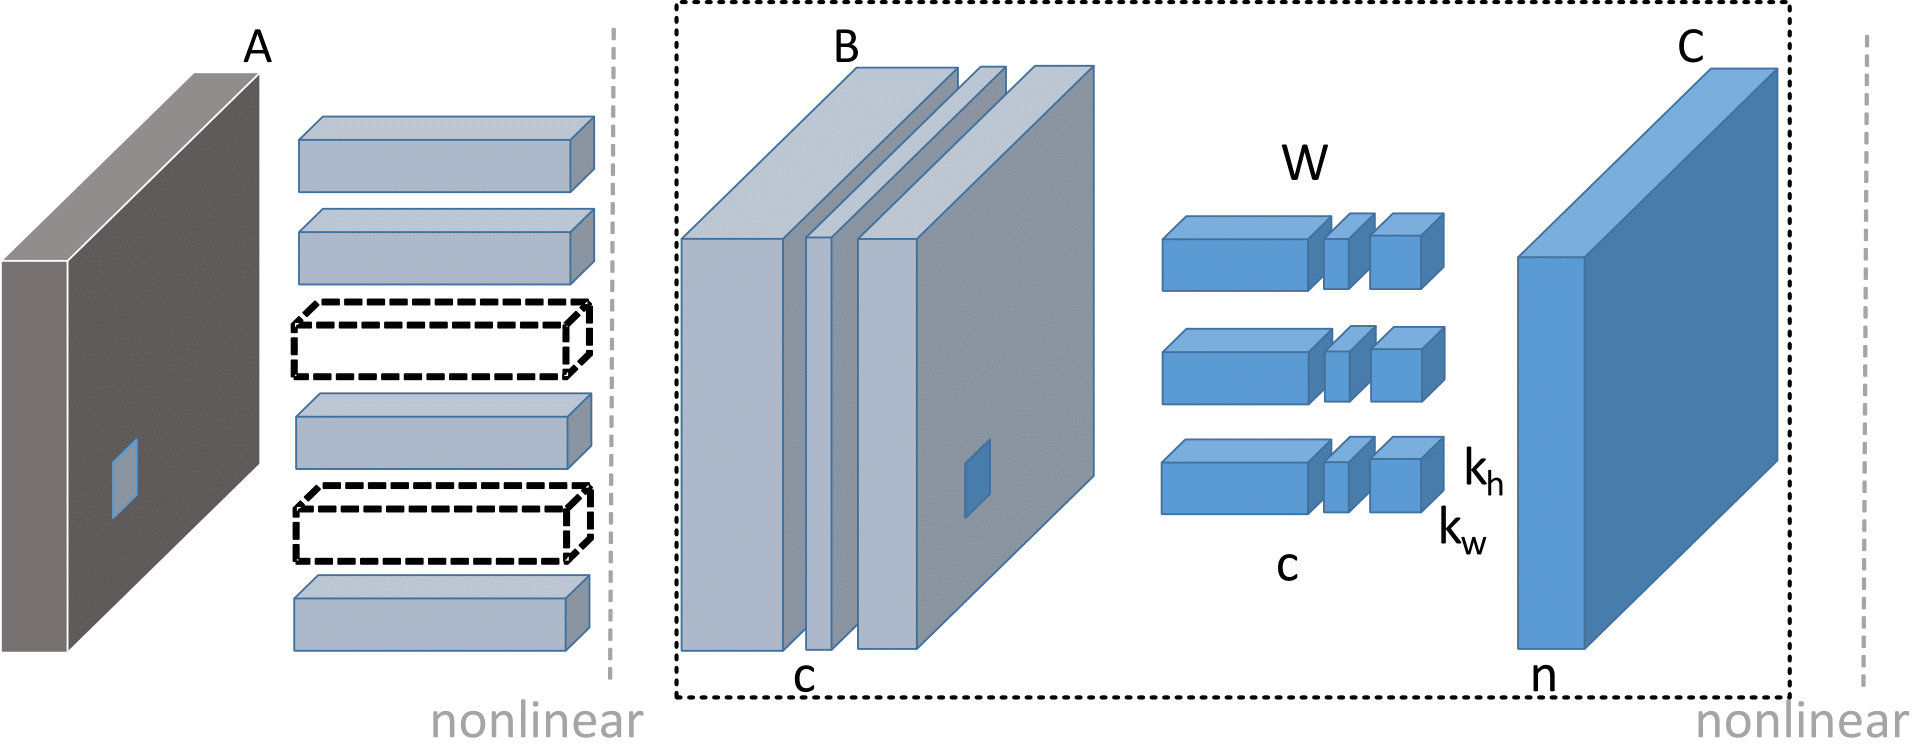
\includegraphics[width=8cm]{images/pruning/channel_pruning.png}
    \centering
    \caption{Channel pruning for accelerating a CNN}\label{fig:channel_pruning}
\end{figure}

The first is the channel selection, since a proper channel combination to
maintain as much information needs to be selected.
The second is reconstruction. The following feature maps need to be
reconstructed using the selected channels. Motivated by this, the process is an
\textit{\textbf{iterative two-step algorithm}}.

In the first step, the aim is to \textit{select most representative channels}.
Since an exhaustive search is infeasible even for tiny networks, a LASSO
regression based method needs to be performed to figure out representative
channels and prune redundant ones.

In the second step, \textit{outputs are reconstructed with remaining channels}
with linear least squares.

The whole model can be pruned applying the approach layer by layer
sequentially. For each layer, input volumes are obtained from the current input
feature map, and output volumes from the output feature map of the un-pruned
model.\cite{He_2017}

\subsubsection{Structured Pruning}
Pruning techniques can be broadly categorized as structured or unstructured.
\textit{Unstructured pruning} does not follow a specific geometry or
constraint. In most cases, this technique needs extra information to represent
sparse locations. It depends on sparse representation for computational
benefits.
On the other hand, \textit{structured sparsity} places non-zero parameters at
well-defined locations. This kind of constraint enables modern CPUs and
graphics processing units (GPUs) to easily exploit computational savings.

\begin{figure}[ht]
    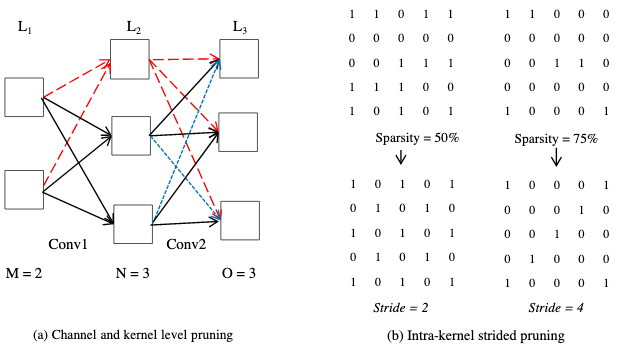
\includegraphics[width=\textwidth]{images/pruning/structured_pruning.png}
    \centering
    \caption{Structured pruning}\label{fig:structured_pruning}
\end{figure}

Channel, kernel and intra-kernel sparsity could be a mean of \textit{structured
pruning}. In \textit{channel level pruning}, all the incoming and outgoing
weights to/from a feature map are pruned. Channel level pruning can directly
produce a lightweight network.
\textit{Kernel level pruning} drops a full k × k kernel, whereas the
intra-kernel sparsity prunes weights in a kernel. The intra kernel strided
sparsity can significantly speed-up convolution layer processing.
The kernel level pruning is a special case of \textit{intra-kernel sparsity}
with 100\% pruning. These granularities can be applied in various combinations
and different orders.\cite{Anwar_2017}

\subsection{Pruning pipeline}
So far I've been explaining what pruning is and what kind of techniques exist
to pruning neural networks. Let's take a step back and see how these techniques
fit the big picture of the pruning pipeline.
There are different ways to apply pruning to neural networks:

\subsubsection{Traditional network pruning pipeline}

This is the traditional approach for pruning a neural network. It prunes
redundant connections using a three-step method:
\begin{enumerate}
    \item Train the network to learn which connections are important: unlike
        conventional training, the final values of the weights are not learnt,
        but rather which connections are important.
    \item Prune the unimportant connections: all connections with weights below
        a threshold are removed from the network, converting a dense network
        into a sparse network.
    \item Retrain the network to fine tune the weights of the remaining
        connections: that's the critical step because if the pruned network is
        used without retraining, accuracy is significantly impacted.
\end{enumerate}

Learning the right connections is an \textbf{iterative process}. Pruning
followed by a retraining is one iteration, after many such iterations the
minimum number connections could be found.

\begin{figure}[ht]
    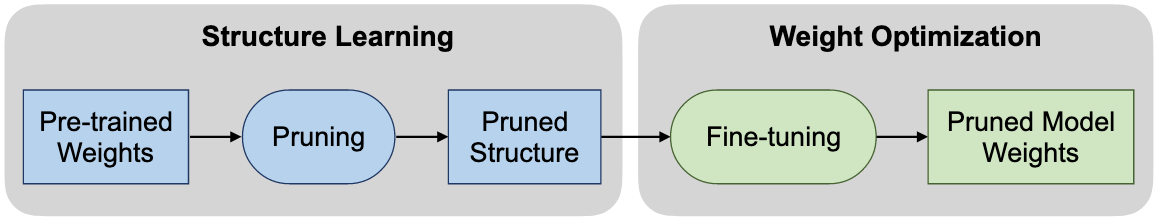
\includegraphics[width=\textwidth]{images/pruning/traditional_pipeline.png}
    \centering
    \caption{Traditional pruning pipeline}\label{fig:traditional_pipeline}
\end{figure}

After pruning connections, neurons with zero input connections or zero output
connections may be safely pruned. This pruning is furthered by removing all
connections to or from a pruned neuron. The retraining phase automatically
arrives at the result where dead neurons will have both zero input connections
and zero output connections.
This occurs due to gradient descent and regularization. A neuron that has zero
input connections (or zero output connections) will have no contribution to the
final loss, leading the gradient to be zero for its output connection (or input
connection), respectively.
Only the regularization term will push the weights to zero. Thus, the dead
neurons will be automatically removed during retraining.~\cite{han2015learning}

In this thesis we will focus mainly on the traditional pipeline but the
described approach can be easily applied to other pruning pipelines.

\subsubsection{Training from scratch}
Another pruning pipeline is ``training from scratch'' where the network pruning
is rethought.
Generally, there are two common assumed beliefs behind this pruning procedure.
First, it is assumed that starting with training a large, over-parametrized
network is important as it provides a high-performance model (due to stronger
representation \& optimization power) from which one can safely remove a set of
redundant parameters without significantly affecting the accuracy. Therefore,
this is usually believed, and reported to be superior to directly training a
smaller network from scratch \- a commonly used baseline approach.
Second, both the pruned architecture and its associated weights are assumed to
be essential for obtaining the final efficient model. Thus most existing
pruning techniques choose to fine-tune a pruned model instead of training it
from scratch. The preserved weights after pruning are usually considered to be
critical.

\begin{figure}[ht]
    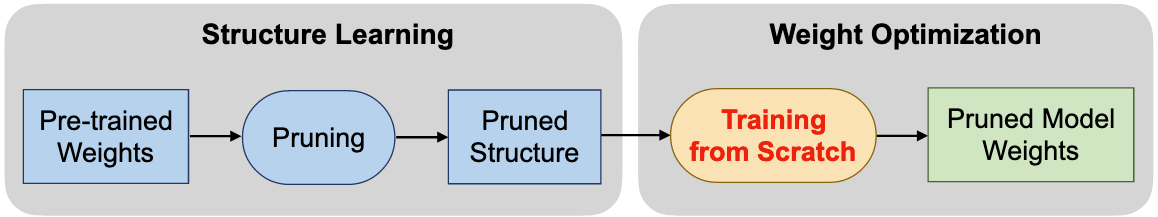
\includegraphics[width=\textwidth]{images/pruning/liu_pipeline.png}
    \centering
    \caption{Pruning pipeline with training from scratch}\label{fig:liu_pipeline}
\end{figure}

With training from scratch, both of the beliefs mentioned above are not
necessarily true for structured pruning methods, which prune at the levels of
convolution channels or larger.
For structured pruning methods with predefined target network architectures,
directly training the small target model from random initialization can achieve
the same, if not better, performance, as the model obtained from the
three-stage pipeline.
For structured pruning methods with auto-discovered target networks, training
the pruned model from scratch can also achieve comparable or even better
performance than fine-tuning.
Interestingly, for unstructured pruning method that prunes individual
parameters, training from scratch can mostly achieve comparable accuracy with
pruning and fine-tuning on smaller-scale datasets, but fails to do so on the
large-scale ImageNet benchmark.
Note that in some cases, if a pre-trained large model is already available,
pruning and fine-tuning from it can save the training time required to obtain
the efficient model.~\cite{liu2018rethinking}

\subsubsection{Pruning from scratch}
In this pipeline, pre-training an over-parametrized model is not necessary
step for obtaining the target pruned structure. In fact, a fully-trained
over-parametrized model will reduce the search space for the pruned structure.

Is it necessary for learning the pruned model structure from pre-trained
weights?
After some research it has been found that the answer is quite surprising: an
effective pruned structure does not have to be learned from pre-trained
weights~\cite{Wang_2020}.

It has been empirically shown that the pruned structures discovered from
pre-trained weights tend to be homogeneous, which limits the possibility of
searching for better structure.

In  fact, more diverse and effective pruned structures can be discovered by
directly pruning from randomly initialized weights, including  potential models
with better performance. Based  on  the  above  observations, it has been
created a novel network pruning pipeline where a pruned network structure can
be directly learned from the randomly initialized weights (see
\autoref{fig:scratch_pipeline}). This pruning pipeline allows \textbf{pruning
from scratch.}

\begin{figure}[ht]
    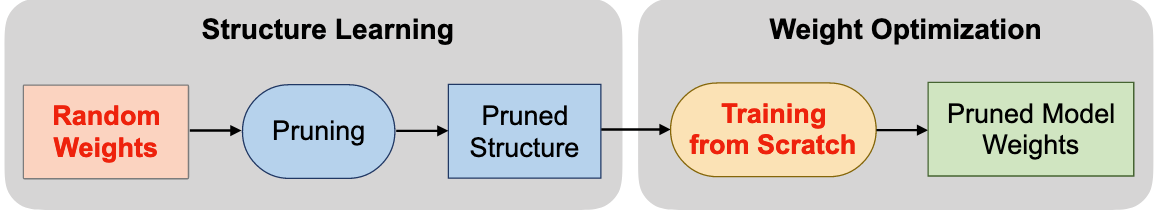
\includegraphics[width=\textwidth]{images/pruning/scratch_pipeline.png}
    \centering
    \caption{Pruning pipeline with pruning from scratch}\label{fig:scratch_pipeline}
\end{figure}

Specifically, it is used a similar technique in Network Slimming to learn the
channel importance by associating scalar gate values with each layer.
The channel importance is optimized to improve the model performance under the
sparsity regularization.
What is different from previous works is that random weights are not updated
during this process. After finishing the learning of channel importance, a
simple binary search strategy is used to determine the channel number
configurations of the pruned model given resource constraints (e.g., FLOPS).
Since it is not needed to update the model weights during optimization, the
pruned structure can be discovered at an extremely fast speed.

This approach not only greatly reduces the pre-training burden of traditional
pruning methods, but also achieves similar or even higher accuracy under the
same computation budget.~\cite{Wang_2020}

\subsection{Pruning-Accuracy trade-offs}\label{subsec:tradeoff}
When a neural network is pruned, its structure and architecture might change
affecting various characteristic. Pruning affects mostly sparsity of the model
and this has an effect on model size, memory used for inference, number of
parameters, speed and latency, compute power and energy needed for
interference.
Whilst pruning has mostly a positive impact on the above metrics, this
optimization might have a negative impact on accuracy of the network model. Of
course, the drop in accuracy needs to be limited or removed completely and
there are techniques for doing so.
In the section though, I will focus on the trade-offs which need to be
considered when pruning a network model.

\begin{figure}[ht]
    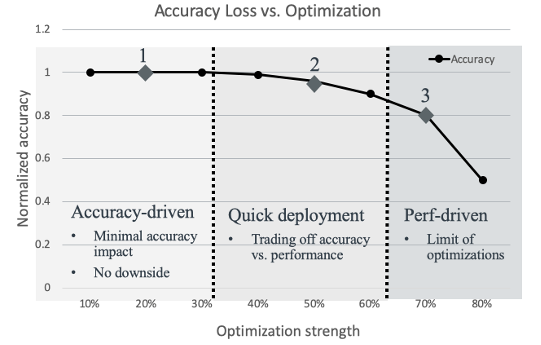
\includegraphics[width=11cm]{images/pruning/tradeoff.png}
    \centering
    \caption{Trade-off between accuracy and optimization strength}\label{fig:tradeoff}
\end{figure}

As the model sparsity increases, a well-designed pruning technique can
efficiently reduce the parameter redundancy while maintaining the original
accuracies. However, after the over-parametrization has been exploited, pruning
or any other model optimization technique will start to introduce accuracy
degradations which are traded for higher optimization strength and better
inference performance. Three typical scenarios are illustrated in \autoref{fig:tradeoff}

\begin{itemize}
    \item \textbf{Accuracy-driven}: in this region, the optimizations produce
        minimal accuracy impact with no downside.
    \item \textbf{Quick deployment}: the trade-off between accuracy and
        performance is the key in this region.
    \item \textbf{Performance-driven}: this region represents the deployment on
        highly resource-constrained devices where the limit of optimizations is
        reached.
\end{itemize}

Accuracy usually is measured with Top-1 and/or Top-5 terms. These are:
\begin{itemize}
    \item \textbf{Top-1}: the answer given by the model must be exactly the
        expected one. In case of classification, it is the answer with highest
        probability. It is the conventional accuracy.
    \item \textbf{Top-5}: the expected answer is any of the first five answers
        with highest probability.
\end{itemize}

When calculating accuracy, Top-1/5 are used to compare against other metrics.
Depending where the model is needed for, a different levels of optimizations is
needed and they might target different kinds of metrics.
Pruning is one of those techniques which affect any aspect of the neural
network: model size, memory used, latency etc

It can be more or less aggressively tuned depending what level of optimization
the network needs to have.
When pruning a neural network, due its over-parametrized and redundant nature,
a usual target sparsity could be between 50\% and 80\%.
These values though depend from the model used and the result of the
evaluation, hence they can be more than 80\% as well.

\section{An overview of pruning in TensorFlow Model Optimization}\label{sec:pruningtfmot}
In this section I will explain briefly how pruning is implemented in TensorFlow
Model Optimization (TFMOT).

TFMOT already supports pruning as technique to optimize neural network and
\textbf{sparsity} is the module that deals with pruning.

\begin{lstlisting}[language=Python, label={lst:tfmotpruningapi},
    caption=Pruning API in TFMOT]
import tensorflow_model_optimization as tfmot

model = build_your_model()

pruning_schedule = tfmot.sparsity.keras.PolynomialDecay(
    initial_sparsity=0.0,
    final_sparsity=0.5,
    begin_step=2000,
    end_step=4000)

model_for_pruning = tfmot.sparsity.keras.prune_low_magnitude(
    model,
    pruning_schedule=pruning_schedule)

|*\ldots*|

model_for_pruning.fit(|*\ldots*|)
\end{lstlisting}

There are few things to explain in \autoref{lst:tfmotpruningapi}. At the time
of writing TFMOT supports two \textbf{pruning schedules}:

\begin{itemize}
    \item \texttt{ConstantSparsity}: this schedule applies constant sparsity
        (\%) throughout training.
    \item \texttt{PolynomialDecay}: this schedule applies pruning based on a
        polynomial function, so it is non-constant.
\end{itemize}

Both pruning schedules are taking the following parameters:

\begin{itemize}
    \item \texttt{final/target\_sparsity}: this is the sparsity the network
        should have once the training has ended.
    \item \texttt{begin\_step}: step at which to begin pruning.
    \item \texttt{end\_step}: step at which to end pruning (-1 means to prune
        till the end of training).
    \item \texttt{frequency}: only apply pruning every \texttt{frequency} step.
\end{itemize}

The \texttt{PolynomialDecay} accepts a couple of extra parameters:

\begin{itemize}
    \item \texttt{initial\_sparsity}: sparsity (\%) at which pruning begins.
    \item \texttt{power}: exponent to be used in the sparsity function.
\end{itemize}

Which schedule to use? It seems there has not been much research on what
pruning schedule to use depending on the condition.
It is known that PolynomialDecay applies the pruning gradually: if the pruning
is applied later in the training, the network has time to converge leading to
more robust and stable results.
The same can be applied with ConstantSparsity since the pruning starts, the
sparsity will be applied straight away and this might cause some instability in
the results.
The best way to choose the schedule is through experimentation.

\subsection{Pruning API in TFMOT}
Pruning API in TFMOT are very easy to use. Below a more detailed example that
shows how to prune a model. I skip the details of building the model and focus
more on the pruning. In \autoref{sec:mnistpipeline} I'll show details on how to
create a model.

\begin{lstlisting}[language=Python, label={lst:tfmotpruningexample},
    caption=Pruning example in TFMOT]
import tempfile
import os

import tensorflow as tf
import numpy as np

from tensorflow import keras
import tensorflow_model_optimization as tfmot

# Load MNIST dataset
mnist = keras.datasets.mnist
(train_images, train_labels), (test_images, test_labels) = mnist.load_data()

# Normalize the input image so that each pixel value is between 0 to 1.
train_images = train_images / 255.0
test_images = test_images / 255.0

# Build and train the model
model = build_and_train_your_model()

prune_low_magnitude = tfmot.sparsity.keras.prune_low_magnitude

# Compute end step to finish pruning after 2 epochs
batch_size = 128
epochs = 2

# 10% of training set will be used for validation set
validation_split = 0.1

num_images = train_images.shape[0] * (1 - validation_split)
end_step = np.ceil(num_images / batch_size).astype(np.int32) * epochs

# Define pruning parameters
pruning_params = {
  "pruning_schedule": tfmot.sparsity.keras.PolynomialDecay(
    initial_sparsity=0.4,
    final_sparsity=0.8,
    begin_step=0,
    end_step=end_step)
}

model_for_pruning = prune_low_magnitude(model, **pruning_params)

# "prune_low_magnitude" requires a recompile
model_for_pruning.compile(
  optimizer='adam',
  loss=tf.keras.losses.SparseCategoricalCrossentropy(from_logits=True),
  metrics=['accuracy']
)

logdir = tempfile.mkdtemp()

callbacks = [
  tfmot.sparsity.keras.UpdatePruningStep(),
  tfmot.sparsity.keras.PruningSummaries(log_dir=logdir),
]

# Fine tune with pruning for two epochs
model_for_pruning.fit(
  train_images,
  train_labels,
  batch_size=batch_size,
  epochs=epochs,
  validation_split=validation_split,
  callbacks=callbacks
)

# Evaluate the accuracy of the pruned model
_, model_for_pruning_accuracy = model_for_pruning.evaluate(
  test_images,
  test_labels,
  verbose=0
)
print('Pruned test accuracy:', model_for_pruning_accuracy)
\end{lstlisting}

The \autoref{lst:tfmotpruningexample} can be divided in the following three
sections:

\begin{enumerate}
    \item Define and train the model (lines 1--31)
    \item Setup the model pruning (lines 33--49)
    \item Prune, fine tuning weights and evaluate the model (lines 51--74)
\end{enumerate}

Below more details of the three sections.

\subsubsection{Define and train the model}
Apart the usual imports at the top of the file, the
MNIST\footnote{\url{http://yann.lecun.com/exdb/mnist/}} dataset is loaded
generating the split between training and test images (line 12).
10\% of the dataset is kept for validation purposes (line 28)

\texttt{build\_and\_train\_your\_model} is a custom function to define and
train the model.

\texttt{batch\_size = 128} defines the number of samples that will be
propagated through the network. In this case 128 samples at the time are taken
and propagated through the network.
The main advantage is the memory usage: the memory footprint is the equivalent
of loading 128 samples of the training data at any time.

\texttt{epochs = 2} means that the training will do a full pass twice over the
full training set. Please note that in this case the epochs defines how many
passes the pruning training will do.

Finally the number if images are the full set minus 10\% reserved to
validation (line 30). The shape of \texttt{train\_images} is the following

\begin{lstlisting}[language=Python, caption=Shape of train\_images]
>>> train_images.shape
(60000, 28, 28)
\end{lstlisting}

The first element is the number if images present in the dataset.

With all data above, the \texttt{end\_step} is then calculated.

\subsubsection{Setup the model pruning}
In this block, the model is prepared for the pruning activity.
This is done by defining the pruning parameters. In this case only the pruning
schedule has been defined (lines 34--40).

\texttt{prune\_low\_magnitude} accepts as parameters the trained model and the
dictionary with the pruning settings: the function has the goal to augment the
model layers with pruning information taken by the pruning parameters.
The resulting model then is compiled again (lines 45--49) before calling the
\texttt{fit} method.

\subsubsection{Prune, fine tuning weights and evaluate the model}
After the compilation of the model, it is finally time to prune the model.

The \texttt{UpdatePruningStep} callback is the one that updates pruning
wrappers with the optimizer step. Not adding this callback to the \texttt{fit}
method will result in throwing an error.

Finally the \texttt{fit} method fine-tunes the weights thanks to the callbacks
definition above.
After the pruning, the model is evaluated and return the accuracy of the new
model (lines 69--74)
